\documentclass[11pt]{article}
\usepackage{fullpage}
\usepackage{amsmath, amsfonts}
\usepackage[utf8]{inputenc}

\usepackage{graphicx}
\graphicspath{ {images/} }

\begin{document}
\begin{center}
{{\Large \sc Introduction to Machine Learning and Data Mining}} \newline	
{{\Large \sc Forest fires}}
\end{center}
\rule{\textwidth}{1pt}
\begin{description}
\item[Student names and ids:] Anders H. Opstrup (s160148); Gu Jinshan (s161944)
\item[Report:] 1
\end{description}
\rule{\textwidth}{1pt}

% 1. Description of our data set.
\section{Description of the data set}
This section of the report will shed some light on basic information about the dataset used in the project. The dataset is a collection of forest fires. The goal of the data is to try to predict forest fries in an attempt to prevent casualties and property damages. A further description of the attributes in the dataset can be found in detailed explanation section of the report.

\subsection{Place of data}
The data is obtained from this link: http://archive.ics.uci.edu/ml/datasets/Forest+Fires

\subsection{Previously work on the data set}
P. Cortez and A. Morais. A Data Mining Approach to Predict Forest Fires using Meteorological Data.
In Proceedings of the 13th EPIA 2007 - Portuguese Conference on Artificial Intelligence, 
December, 2007. (http://www.dsi.uminho.pt/~pcortez/fires.pdf) \newline

In the above reference, the output "area" was first transformed with a ln(x+1) function.
Then, several Data Mining methods were applied. After fitting the models, the outputs were
post-processed with the inverse of the ln(x+1) transform. Four different input setups were
used. The experiments were conducted using a 10-fold (cross-validation) x 30 runs. Two
regression metrics were measured: MAD and RMSE. A Gaussian support vector machine (SVM) fed
with only 4 direct weather conditions (temp, RH, wind and rain) obtained the best MAD value:
12.71 +- 0.01 (mean and confidence interval within 95\% using a t-student distribution). The
best RMSE was attained by the naive mean predictor. An analysis to the regression error curve
(REC) shows that the SVM model predicts more examples within a lower admitted error. In effect,
the SVM model predicts better small fires, which are the majority.

\subsection{Primary machine learning modeling aim}
Detection and test of outlier methods and try different regression methods and look at the correlation between the temperature, wind, rain and the burn area. 


% 2. Detailed explanation of the attributes of the data.
\section{A detailed explanation of the attributes of the data}

\subsection*{Describe if the attributes are discrete/continous, Nominal/Ordinal/Interval/Ratio.}
	\begin{enumerate}
	\item X - Discrete, Nominal
	\item Y - Discrete, Nominal
	\item month - Discrete, Ordinal
	\item day - Discrete, Ordinal
	\item FFMC - Continous, Interval
	\item DMC - Continous, Interval
	\item DC - Continous, Interval
	\item ISI - Continous, Interval
	\item temp - Continous, Interval
	\item RH - Continous, Ratio
	\item wind - Continous, Ratio
	\item rain - Continous, Ratio
	\item area - Continous, Ratio
	\end{enumerate}
\subsection*{Give an account of whether there are data issues (i.e. missing values or corrupted data) and describe them if so.}
There is no missing values or corrupted data.
\subsection*{Describe the basic summary statistics of the attributes.}
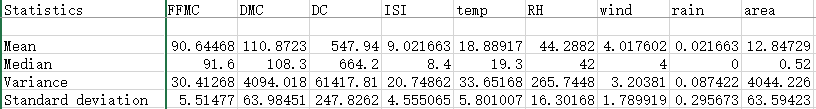
\includegraphics[width=\textwidth]{summary_statistics.png}

% 3. Data visualization(s) based on suitable visualization techniques in- cluding a principal component analysis (PCA).
\section{Data visualization}

The boxplot analyse method have been used for detecting outliers in the data set. In the boxplots below we can see that there are some outliers and some attributes where the dataset is not very detailed. The area attribute needs some stemming for correcting the data, due to a lot of zero areas. The FFMC attribute and ISI also needs stemming for cleaning up the data.

\begin{figure}
\begin{tabular}{cc}
  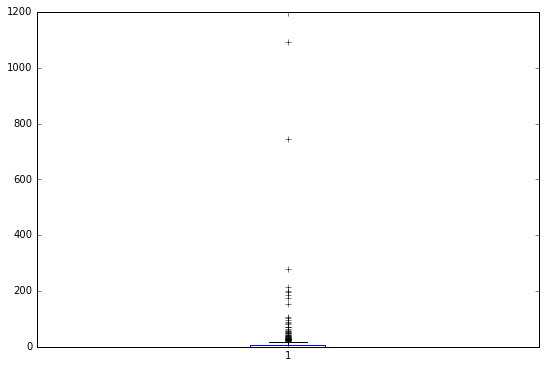
\includegraphics[width=65mm]{images/boxplots/area.png} &   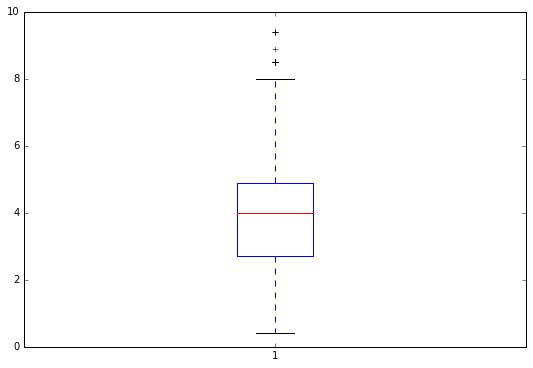
\includegraphics[width=65mm]{images/boxplots/wind.png} \\
(a) area & (b) wind \\[6pt]
 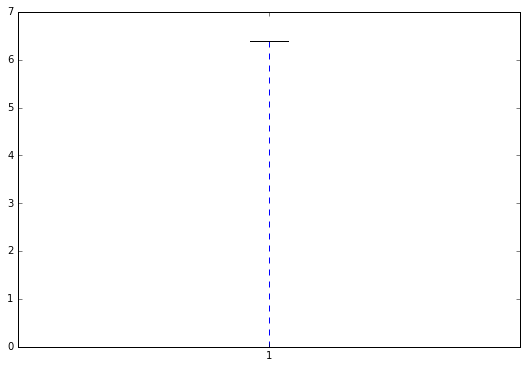
\includegraphics[width=65mm]{images/boxplots/rain.png} &   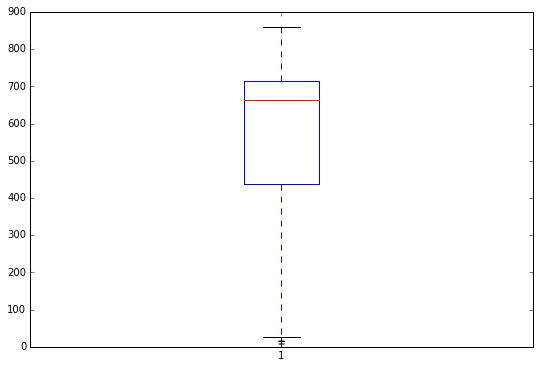
\includegraphics[width=65mm]{images/boxplots/DC.png} \\
(c) rain & (d) DC \\[6pt]
  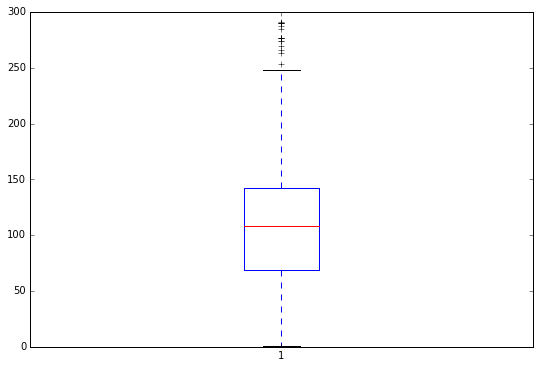
\includegraphics[width=65mm]{images/boxplots/DMC.png} &   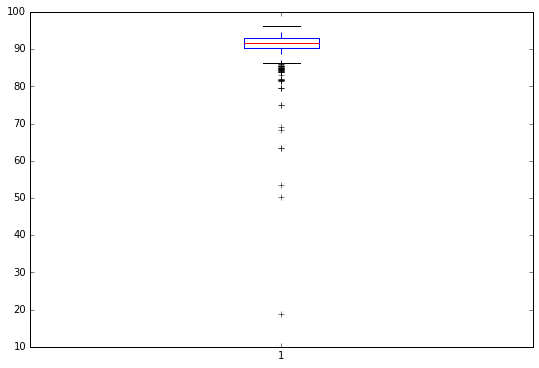
\includegraphics[width=65mm]{images/boxplots/FFMC.png} \\
(e) DMC & (f) FFMC \\[6pt]
\end{tabular}
\caption{Boxplot diagrams}
\end{figure}

\begin{figure}
\begin{tabular}{cc}
 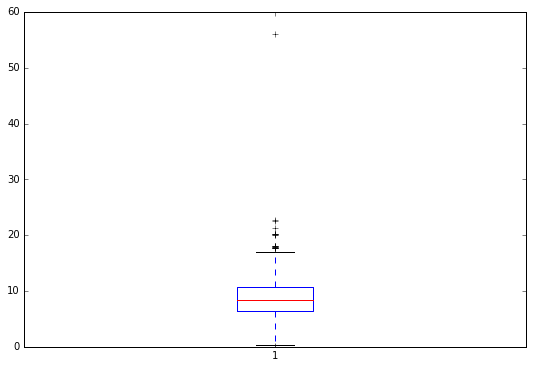
\includegraphics[width=65mm]{images/boxplots/ISI.png} &   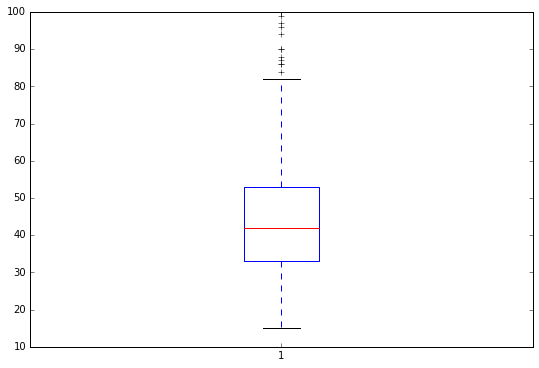
\includegraphics[width=65mm]{images/boxplots/RH.png} \\
(a) ISI & (b) RH \\[6pt]
  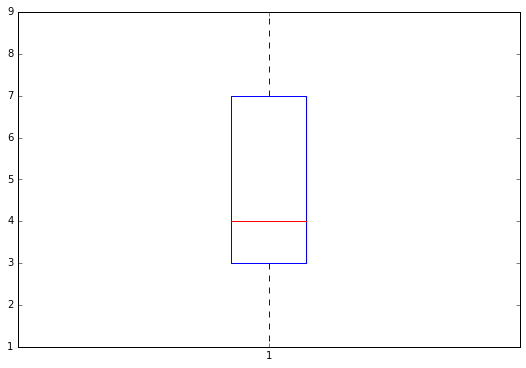
\includegraphics[width=65mm]{images/boxplots/x.png} &   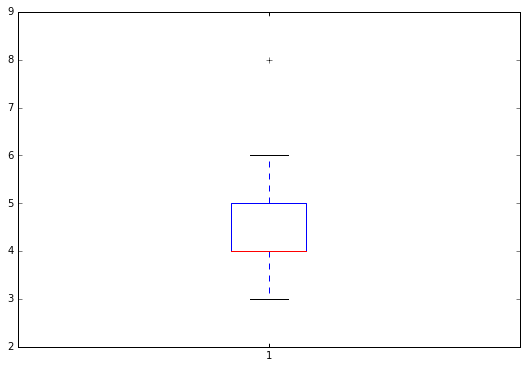
\includegraphics[width=65mm]{images/boxplots/y.png} \\
(c) X & (d) Y \\[6pt]
\multicolumn{2}{c}{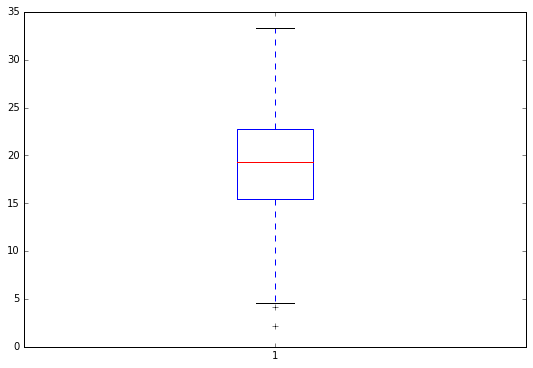
\includegraphics[width=65mm]{images/boxplots/temp.png} }\\
\multicolumn{2}{c}{(e) temp}
\end{tabular}
\caption{Boxplot diagrams}
\end{figure}

\section*{Do the attributes appear to be normal distributed}
We generate the histogram for 9 attributes to find whether the attributes is normal distributed. We did not analysis the attributes X, Y, month and day since it is meaningless draw the histogram for them. From the histogram we can find that the FFMC, ISI and temp attributes seems to be like normal distributed. But others are not. 

\begin{figure}
\begin{tabular}{cc}
  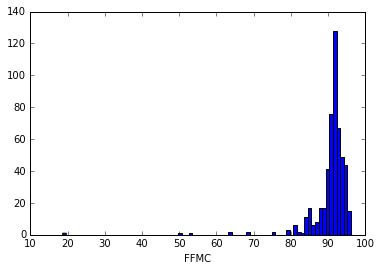
\includegraphics[width=65mm]{images/hist/FFMC.png} &   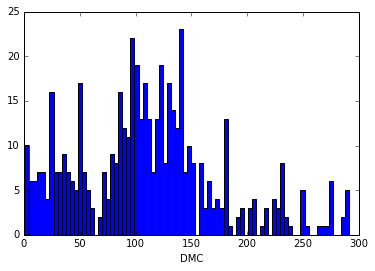
\includegraphics[width=65mm]{images/hist/DMC.png} \\
(a) FFMC & (b) DMC \\[6pt]
 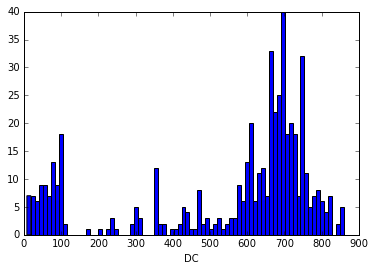
\includegraphics[width=65mm]{images/hist/DC.png} &   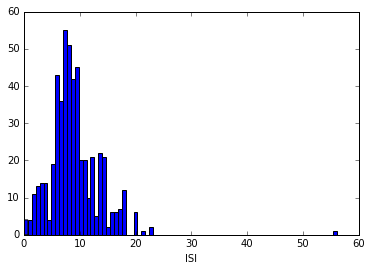
\includegraphics[width=65mm]{images/hist/ISI.png} \\
(c) DC & (d)ISI \\[6pt]

\end{tabular}
\caption{Histogram}
\end{figure}

\newpage

\begin{figure}
\begin{tabular}{cc}
  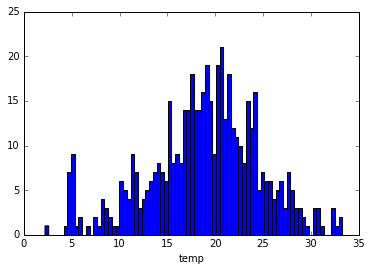
\includegraphics[width=65mm]{images/hist/temp.png} &   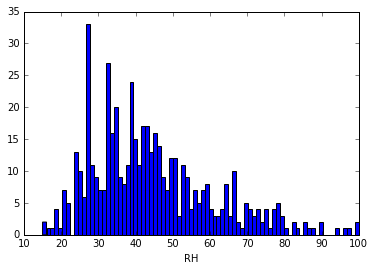
\includegraphics[width=65mm]{images/hist/RH.png} \\
(e) temp & (f) RH \\[6pt]
  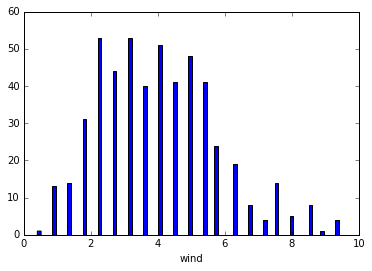
\includegraphics[width=65mm]{images/hist/wind.png} &   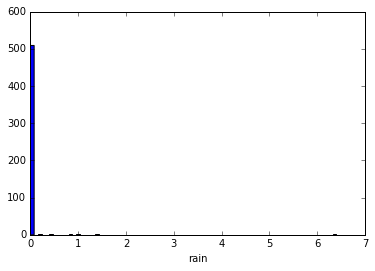
\includegraphics[width=65mm]{images/hist/rain.png} \\
(g) wind & (h) rain \\[6pt]
\multicolumn{2}{c}{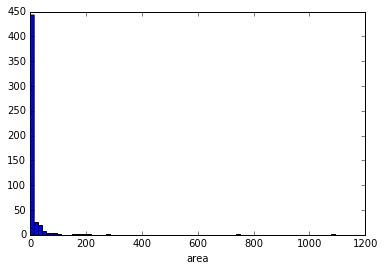
\includegraphics[width=65mm]{images/hist/area.png} }\\
\multicolumn{2}{c}{(i) are}
\end{tabular}
\caption{Histogram}
\end{figure}
\subsection{Variables correlation}
After calculated the C\^{O}R of two variables, we found those two couples of variables are possibly correlated. The absolute value of C\^{O}R are above 0.5. The two scatter plots below show the data distribution.
\begin{figure}[!ht]
\begin{tabular}{cc}
  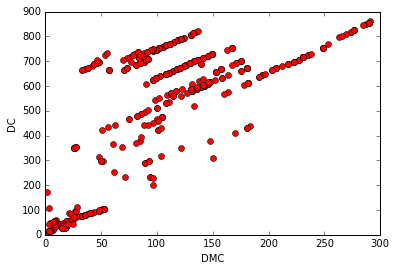
\includegraphics[width=65mm]{fig/correlated/DMC_DC.png} &   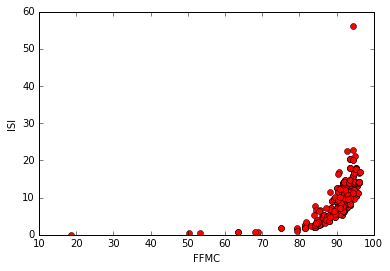
\includegraphics[width=65mm]{fig/correlated/FFMC_ISI.png} \\
(a) C\^{O}R=0.682 & (b) C\^{O}R=0.531 \\[6pt]
\end{tabular}
\caption{ Scatter Plot }
\end{figure}
\section*{PCA}
In order to do the PCA analyse some class had to be made for the dataset. The months was chosen as classes for trying to project the data in aspect of a year. 
By looking at (figure \ref{fig:pca_2}) the reader will see that around 90\% of the information is in component 1, of the PCA model. By this we can conclude that most of the variance happens in the first component and there by is the most important component. 

\vspace{-5pt}
\begin{figure}[H]
	\centering
	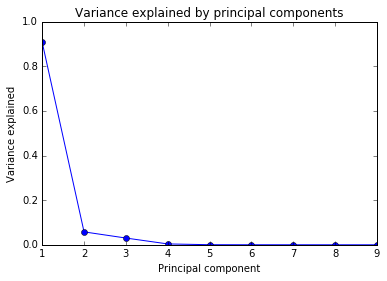
\includegraphics[width=0.7\textwidth]{images/pca/pca_2.png}
	\vspace{-5pt}
	\label{fig:pca_2}
\end{figure}

% 4. Discussion explaining what we have learned about the data.
\section{Discussion}
After analysing the dataset, the group is a bit concerned if the dataset is big enough. With only around 500 records and 11 attributes, the dataset is a bit small. The boxplot shows that there is a lot of outliers in the dataset and no concrete data class where to be found in the dataset, which made the pc-analyse very hard. 

\end{document}